% Options for packages loaded elsewhere
\PassOptionsToPackage{unicode}{hyperref}
\PassOptionsToPackage{hyphens}{url}
%
\documentclass[
  ignorenonframetext,
]{beamer}
\usepackage{pgfpages}
\setbeamertemplate{caption}[numbered]
\setbeamertemplate{caption label separator}{: }
\setbeamercolor{caption name}{fg=normal text.fg}
\beamertemplatenavigationsymbolsempty
% Prevent slide breaks in the middle of a paragraph
\widowpenalties 1 10000
\raggedbottom
\setbeamertemplate{part page}{
  \centering
  \begin{beamercolorbox}[sep=16pt,center]{part title}
    \usebeamerfont{part title}\insertpart\par
  \end{beamercolorbox}
}
\setbeamertemplate{section page}{
  \centering
  \begin{beamercolorbox}[sep=12pt,center]{part title}
    \usebeamerfont{section title}\insertsection\par
  \end{beamercolorbox}
}
\setbeamertemplate{subsection page}{
  \centering
  \begin{beamercolorbox}[sep=8pt,center]{part title}
    \usebeamerfont{subsection title}\insertsubsection\par
  \end{beamercolorbox}
}
\AtBeginPart{
  \frame{\partpage}
}
\AtBeginSection{
  \ifbibliography
  \else
    \frame{\sectionpage}
  \fi
}
\AtBeginSubsection{
  \frame{\subsectionpage}
}
\usepackage{amsmath,amssymb}
\usepackage{iftex}
\ifPDFTeX
  \usepackage[T1]{fontenc}
  \usepackage[utf8]{inputenc}
  \usepackage{textcomp} % provide euro and other symbols
\else % if luatex or xetex
  \usepackage{unicode-math} % this also loads fontspec
  \defaultfontfeatures{Scale=MatchLowercase}
  \defaultfontfeatures[\rmfamily]{Ligatures=TeX,Scale=1}
\fi
\usepackage{lmodern}
\usetheme[]{metropolis}
\ifPDFTeX\else
  % xetex/luatex font selection
\fi
% Use upquote if available, for straight quotes in verbatim environments
\IfFileExists{upquote.sty}{\usepackage{upquote}}{}
\IfFileExists{microtype.sty}{% use microtype if available
  \usepackage[]{microtype}
  \UseMicrotypeSet[protrusion]{basicmath} % disable protrusion for tt fonts
}{}
\makeatletter
\@ifundefined{KOMAClassName}{% if non-KOMA class
  \IfFileExists{parskip.sty}{%
    \usepackage{parskip}
  }{% else
    \setlength{\parindent}{0pt}
    \setlength{\parskip}{6pt plus 2pt minus 1pt}}
}{% if KOMA class
  \KOMAoptions{parskip=half}}
\makeatother
\usepackage{xcolor}
\newif\ifbibliography
\usepackage{graphicx}
\makeatletter
\def\maxwidth{\ifdim\Gin@nat@width>\linewidth\linewidth\else\Gin@nat@width\fi}
\def\maxheight{\ifdim\Gin@nat@height>\textheight\textheight\else\Gin@nat@height\fi}
\makeatother
% Scale images if necessary, so that they will not overflow the page
% margins by default, and it is still possible to overwrite the defaults
% using explicit options in \includegraphics[width, height, ...]{}
\setkeys{Gin}{width=\maxwidth,height=\maxheight,keepaspectratio}
% Set default figure placement to htbp
\makeatletter
\def\fps@figure{htbp}
\makeatother
\setlength{\emergencystretch}{3em} % prevent overfull lines
\providecommand{\tightlist}{%
  \setlength{\itemsep}{0pt}\setlength{\parskip}{0pt}}
\setcounter{secnumdepth}{-\maxdimen} % remove section numbering
\ifLuaTeX
  \usepackage{selnolig}  % disable illegal ligatures
\fi
\usepackage{bookmark}
\IfFileExists{xurl.sty}{\usepackage{xurl}}{} % add URL line breaks if available
\urlstyle{same}
\hypersetup{
  pdftitle={Vergleich verschiedener Dateisysteme für den SD-Karten-Einsatz in eingebetteten Systemen},
  pdfauthor={Michael Kolorz (miko8278@bht-berlin.de)},
  hidelinks,
  pdfcreator={LaTeX via pandoc}}

\title{Vergleich verschiedener Dateisysteme für den SD-Karten-Einsatz in
eingebetteten Systemen}
\author{Michael Kolorz (miko8278@bht-berlin.de)}
\date{4. November 2026}
\institute{Erstprüfer:Prof.~Dr.~Peter Gober ~Zweitprüfer:Prof.~Dr.~David
Dietrich}

\begin{document}
\frame{\titlepage}

\begin{frame}{Themen des Vortrags}
\phantomsection\label{themen-des-vortrags}
\footnotesize

\begin{enumerate}
\tightlist
\item
  Überblick und Motivation
\item
  Hardwaredesign
\item
  Software

  \begin{enumerate}
  \tightlist
  \item
    SPI-SD-Treiber
  \item
    FatFs und littlefs
  \end{enumerate}
\item
  Dateisystemtests

  \begin{enumerate}
  \tightlist
  \item
    Analyse der Schreibfehlerraten mittels bekannter Zeichenfolge
  \item
    Analyse der Schreibfehlerraten mittels bekannter Zeichenfolge und
    manipulierter Schreibfunktion
  \item
    Analyse von pseudo-randomisierter Zeichenfolge bei Anhang an Datei
  \item
    Verhalten der Dateisysteme bei Stromunterbrechungen
  \item
    Direkte Blockadressierung (NoFs)
  \end{enumerate}
\item
  Fazit \normalsize
\end{enumerate}
\end{frame}

\begin{frame}{Überblick}
\phantomsection\label{uxfcberblick}
\end{frame}

\begin{frame}{Motivation persönlich}
\phantomsection\label{motivation-persuxf6nlich}
-test 1 -test 2 ---
\end{frame}

\begin{frame}{Motivation technisch}
\phantomsection\label{motivation-technisch}
-test 3 -test 4
\end{frame}

\begin{frame}{Hardware: Schaltplan}
\phantomsection\label{hardware-schaltplan}
\centering

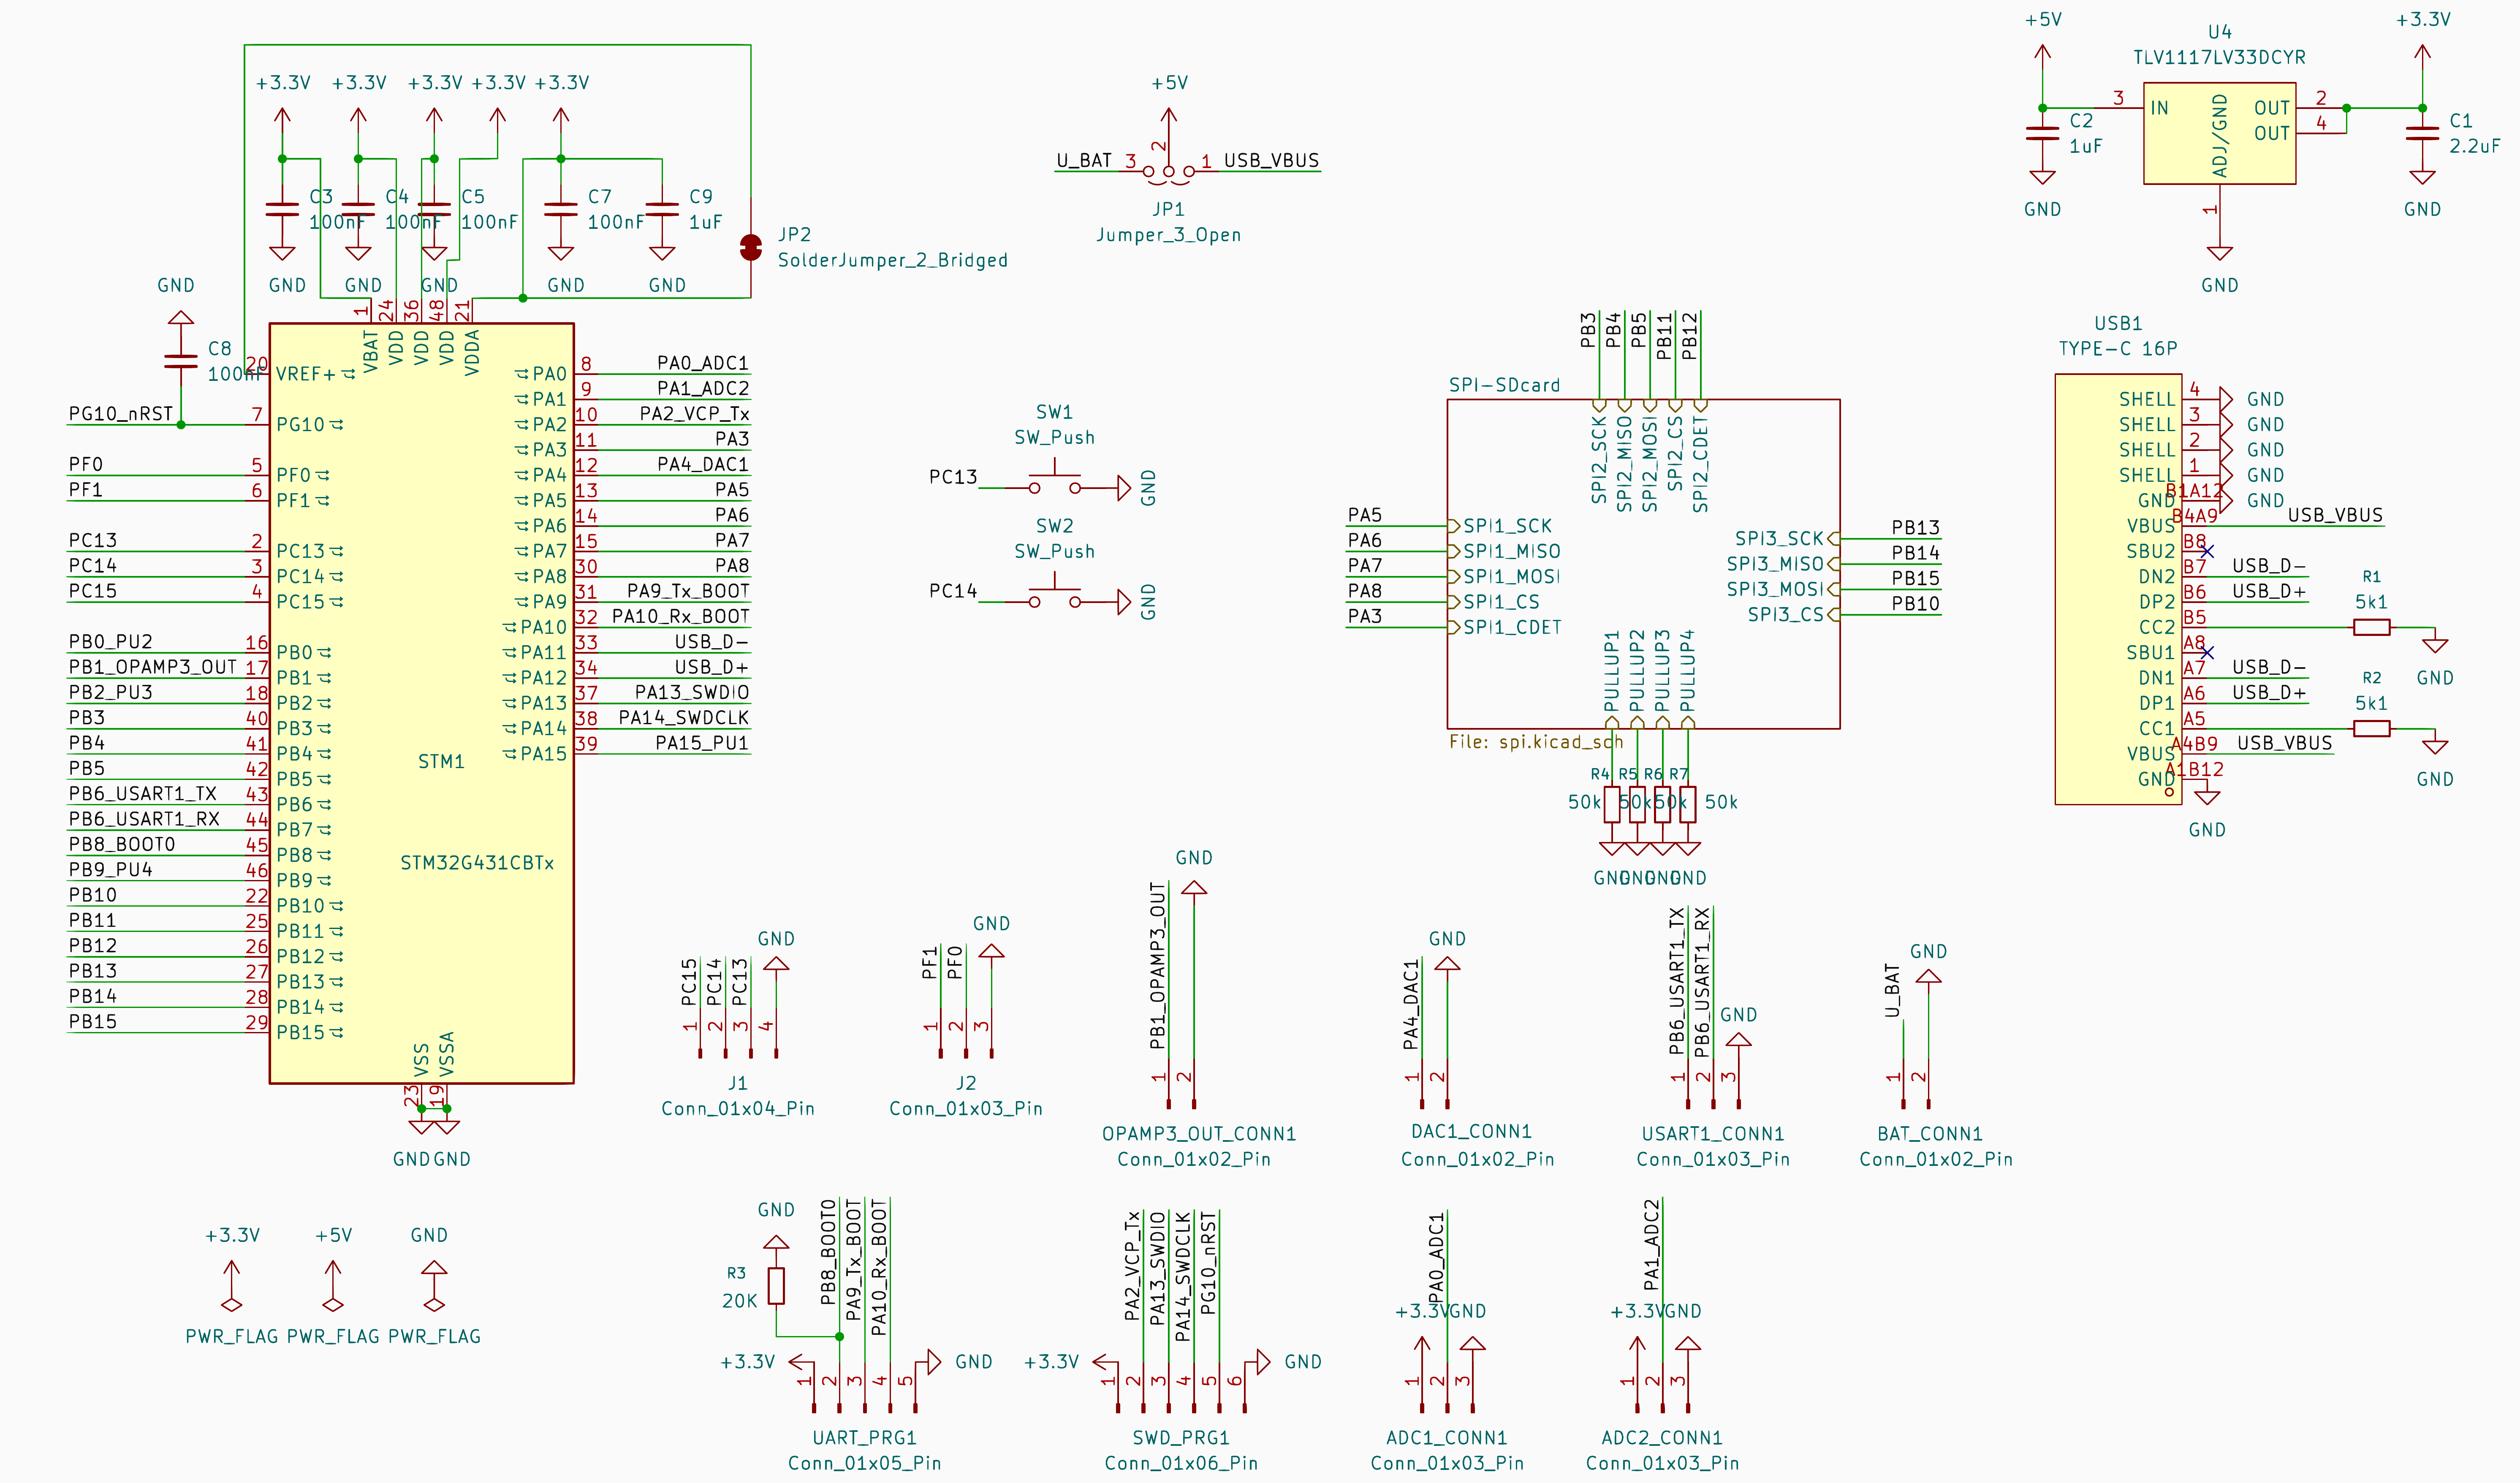
\includegraphics[width=1\textwidth,height=\textheight]{Bilder/Schaltplan_main_highres_grey.png}
\end{frame}

\begin{frame}{Hardware: Platine unbestückt}
\phantomsection\label{hardware-platine-unbestuxfcckt}
\centering

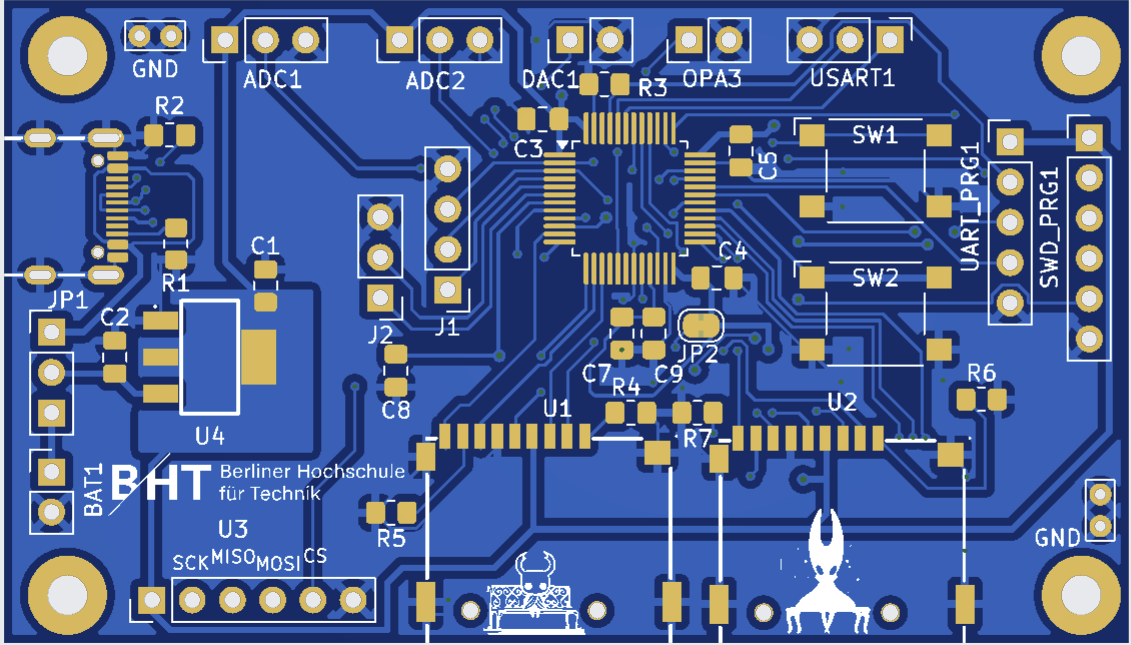
\includegraphics[width=1\textwidth,height=\textheight]{Bilder/PreviewPCB.png}
\end{frame}

\begin{frame}{Hardware: Platine bestückt}
\phantomsection\label{hardware-platine-bestuxfcckt}
\centering

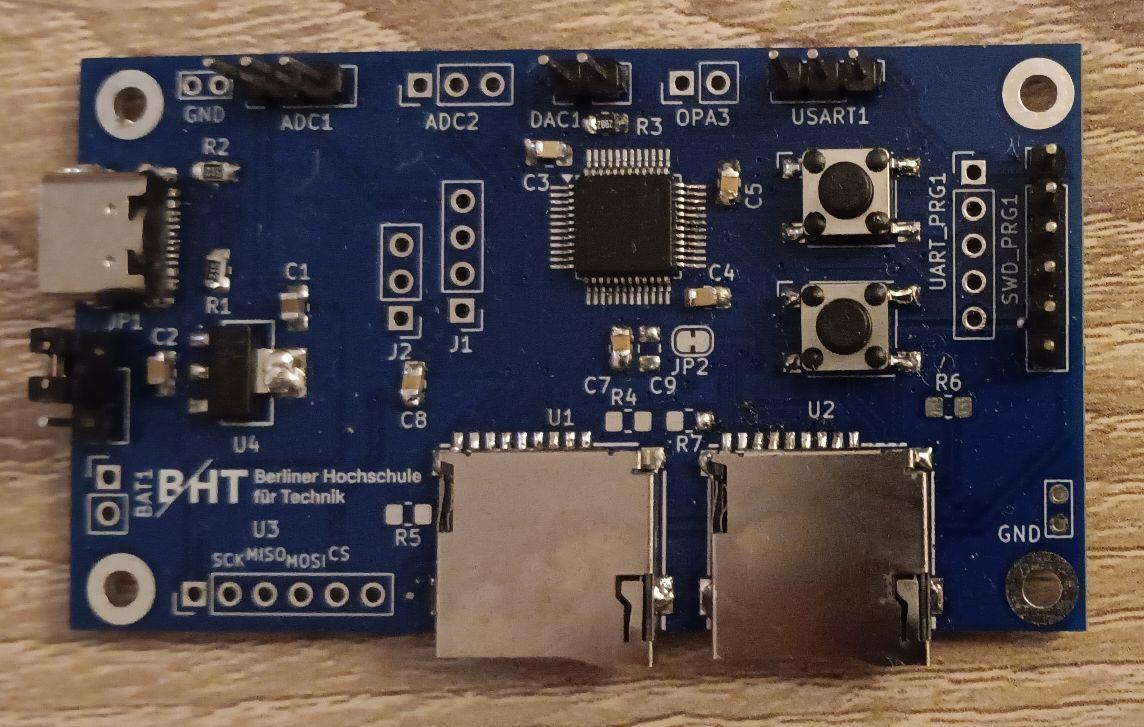
\includegraphics[width=1\textwidth,height=\textheight]{Bilder/Platine_bestueckt.jpg}
\end{frame}

\begin{frame}{Software: SPI-SD-Treiber}
\phantomsection\label{software-spi-sd-treiber}
\end{frame}

\begin{frame}{Software: FatFs}
\phantomsection\label{software-fatfs}
\end{frame}

\begin{frame}{Software: littlefs}
\phantomsection\label{software-littlefs}
\end{frame}

\begin{frame}{Bildertest 2 Nebeneinander}
\phantomsection\label{bildertest-2-nebeneinander}
\begin{columns}[T]
\begin{column}{0.48\textwidth}
\includegraphics[width=1\textwidth,height=\textheight]{Bilder/MISO_dip.png}
\end{column}

\begin{column}{0.48\textwidth}
\includegraphics[width=1\textwidth,height=\textheight]{Bilder/MISO_dip.png}
\end{column}
\end{columns}
\end{frame}

\end{document}
